\documentclass{article}
\usepackage{cmap}
\usepackage{graphicx}
\usepackage{caption}
\usepackage{subcaption}

\usepackage[left=3cm,right=3cm,
    top=2cm,bottom=2cm,bindingoffset=0cm]{geometry}
\linespread{1.5}


\begin{document}
\large
\centerline{}
\vspace*{20pt}
\section{Introduction}
The comparative felidae project aims to perform analysis of gene evolution, evolution of breakpoints and synteny, and also the analysis of selection signatures among the felines. Gene evolution analysis requires a good gene annotation including correct predictions of 5' and 3' UTR regions, exon and intron structure. 
We plan to use TransMap approach from the domestic cat gene annotation to other felines. \\
After an overview of the current available annotations of the domestic cat genome we came to a conclusion that it can be possible to produce a better annotation using Augustus prediction tool guided by the available cat mRNA data. \\
The improvement of the cat's annotation would allow for more precise gene evolution analysis.  In particular, inaccurate stop/start codon predictions as well as errors in splice cite positions and lack of exons may cause artifacts when mapping genes through the species. Another point is that a missing codon may be an evidence for gene divergence. We should provide more confidence that such finding are not the annotation artifacts.\\
Below we summarize the information about the available Felis catus gene annotation resources. We compare the results under consideration that the estimate of the feline gene number is 19000 - 20000, and the number of their alternative isoforms is $\sim$60000.


\section{Available gene annotations}
\subsection{Annotation from \textit{Pontius et al.}}
This annotation (2007) was based on the first draft of cat genome which consisted of the contigs that were aligned with the other available annotated mammalian genomes sequences. The gene predictions were based on pairwise RBM between the aligned sequences that were screened for annotated genes and gene features.

However this annotation was lost so that we were not able to evaluate it’s results. Anyway, this analysis incorporated data and methods that were available in 2007. Since that time the genome assemblies were improved,  and also mapped gene annotations were updated.


\subsection{Annotation from \textit{Tamazian et al.}}
This analysis aimed to identify orthology and find the coding sequences in the cat genome.
The genome features were derived from a comparative gene identification strategy based on RBM search described in \textit{Pontius et al.}.
Due to the aim different from the full gene annotation it lacks the prediction of exact gene structure that would be important for the gene evolution analysis. 

\subsection{Ensembl annotation}
Ensembl gene annotation is based on protein, mRNA, EST, and RNAseq alignments and gene predictions by GeneWise and Exonerate. The cat mRNA and EST sequences were obtained from the GenBank database, the proteins were obtained from the UniProt database. There are $\sim$200 cat proteins in the SwissProt manually curated compartment of the UniProt. However non-cat proteins  were also used in these alignments.\\
According to our estimation this is the best known gene annotation. 
However it has a significant number of errors among the predicted genes beginning with a few nucleotide imprecision (like a \texttt{TT} splice site 2 base pairs off from a regular \texttt{AG} splice site that can be a conserved exon boundary in the other compared mammals) and ending with wrong prediction or loss of exons.\\
The genome browser (http://hgwdev.cse.ucsc.edu) examples of inaccurate gene prediction from this dataset are shown on Figures \ref{fig:missed_exons_mrna_1}, \ref{fig:missed_exons_mrna_2}, \ref{fig:gene_in_ltr}.
We performed an automatic estimation of each reported transcript from this annotation for the following qualities: gaps in coding sequences, CDS and UTR showing unknown and non-canonical splice sites. The transcripts with the identified issues were called erroneous. Next we grouped the overlapping transcripts in order to identify the clusters corresponding to the gene locations. We distinguish the clusters for those that didn’t contain errors in transcripts and those that contained only erroneous transcripts (Table \ref{table:ensembl_refseq_stats}). \\
According to the Table \ref{table:ensembl_refseq_stats} the number of transcripts reported in this annotation is 22{,}656. Whereas the  number of isoforms in mammalian genome is estimated as $\sim$60{,}000 which indicates the incompleteness of the cat gene annotation (Figures \ref{fig:human_mouse_cat_exons}, \ref{fig:human_mouse_cat_exon_density}). The high fragmentation level of predicted exons can be observed on the Figure \ref{fig:human_mouse_cat_exon_density}.

%Figure0
\begin{figure}[h]
\centering
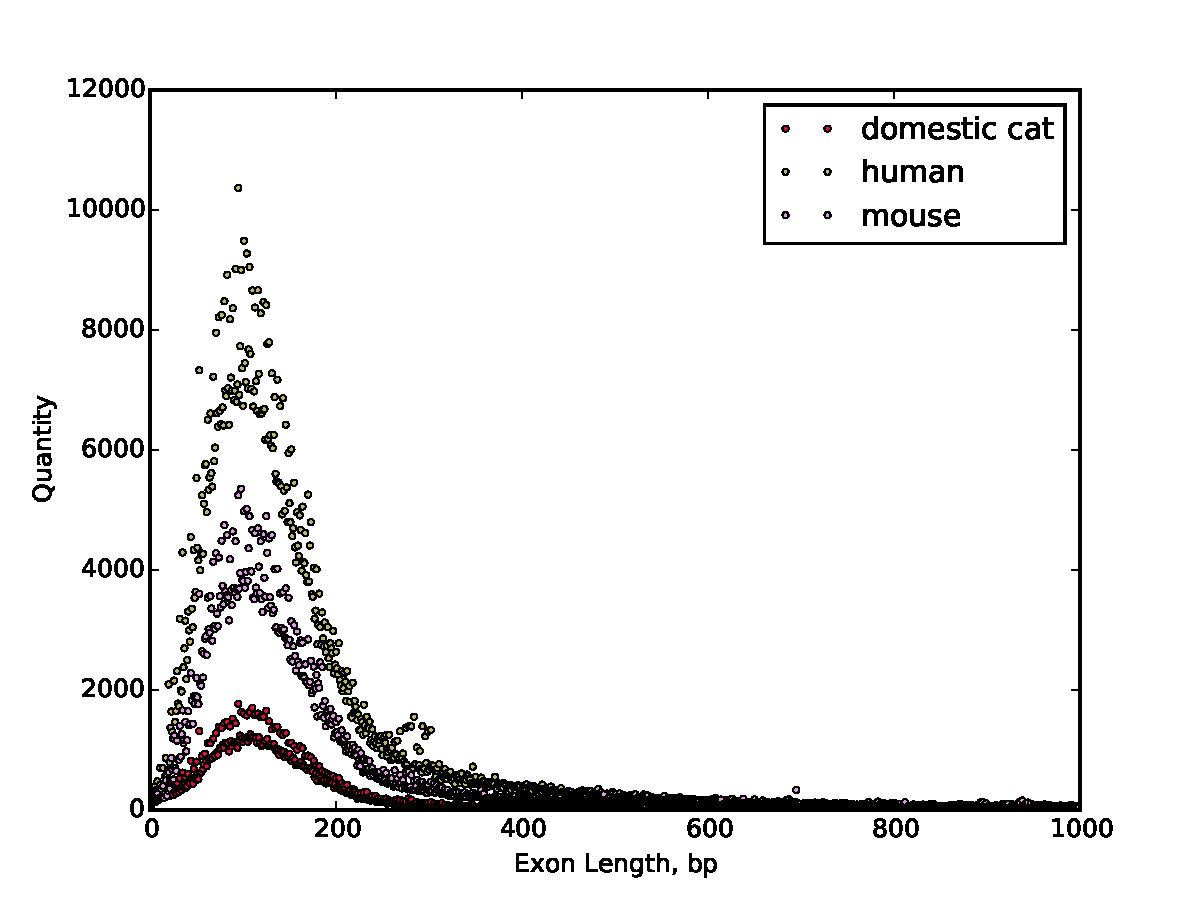
\includegraphics[width=\textwidth]{images/exon_distr_human_mouse_cat.pdf}
\caption{Distribution of exon lengths in mouse (GRCm38), human (GRCh38), and domestic cat (6.2) gene annotations.}
\label{fig:human_mouse_cat_exons}
\end{figure}


%Figure5
\begin{figure}[h]
\centering
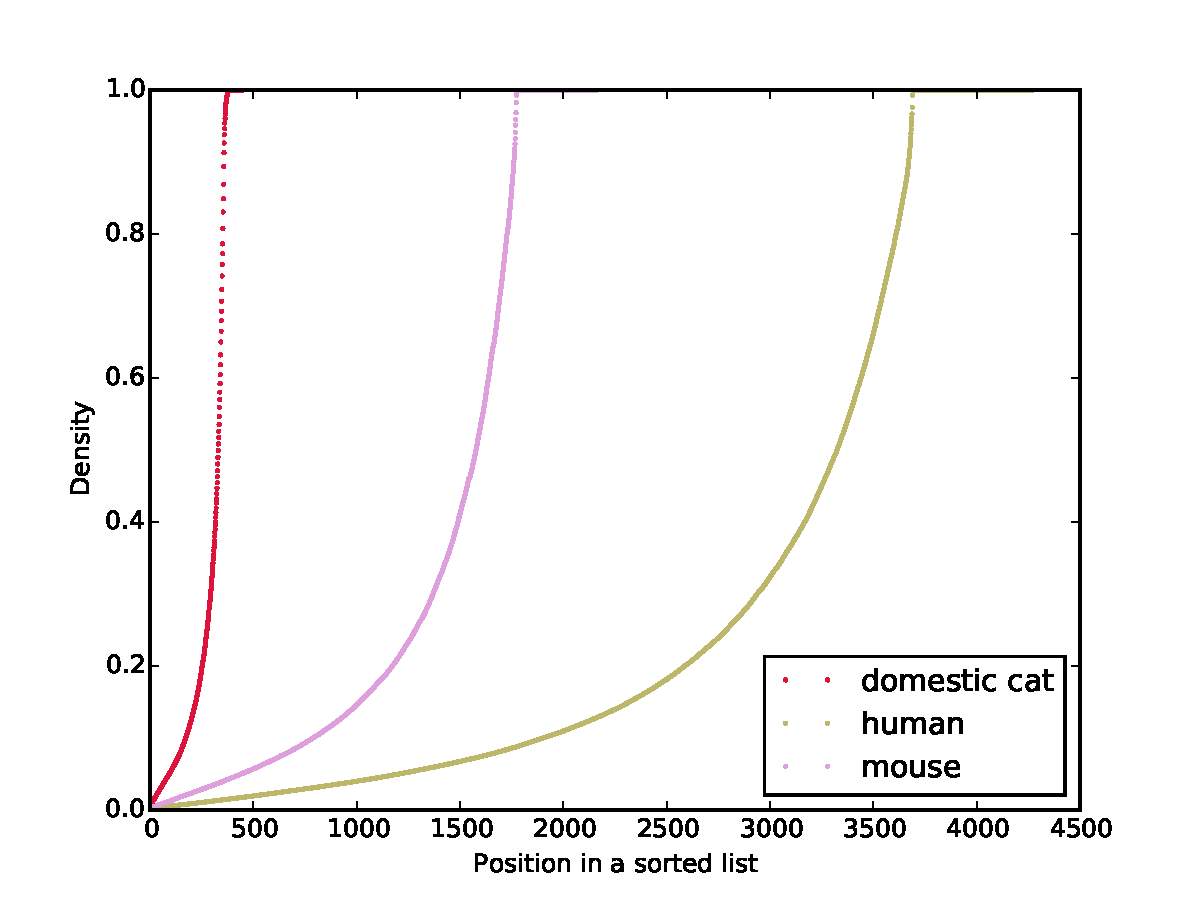
\includegraphics[width=\textwidth]{images/exon_density_human_mouse_cat.pdf}
\caption{For each reported ensembl transcript we calculated the density of identified exons. The lists of exons densities were sorted and compressed by average value in non-overlapping windows of 50 density values. The procedure was performed for mouse (GRCm38), human (GRCh38), and domestic cat (6.2) gene annotations.}
\label{fig:human_mouse_cat_exon_density}
\end{figure}

\textit{Montague et al.} based their research on the ensembl annotation.


%Figure1
\begin{figure}[h]
\centering
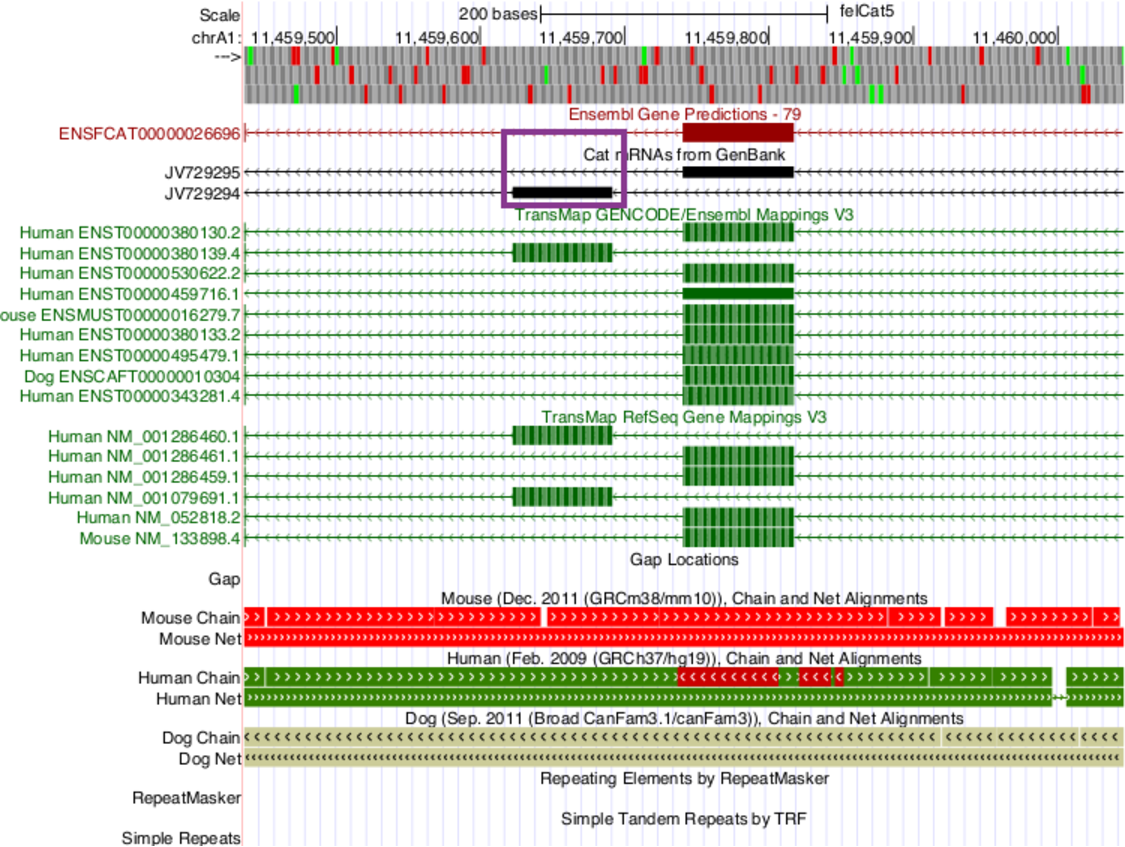
\includegraphics[width=\textwidth]{images/hgt_hgwdev_e926_52a620_edit.pdf}
\caption{According to mRNA track there are two exons in the gene ENSFCAT00000026696, however the annotation lacks prediction of the first exon (marked inside of the purple rectangle). TransMap from other species is able to predict that.}
\label{fig:missed_exons_mrna_1}
\end{figure}

%Figure2
\begin{figure}[h]
\centering
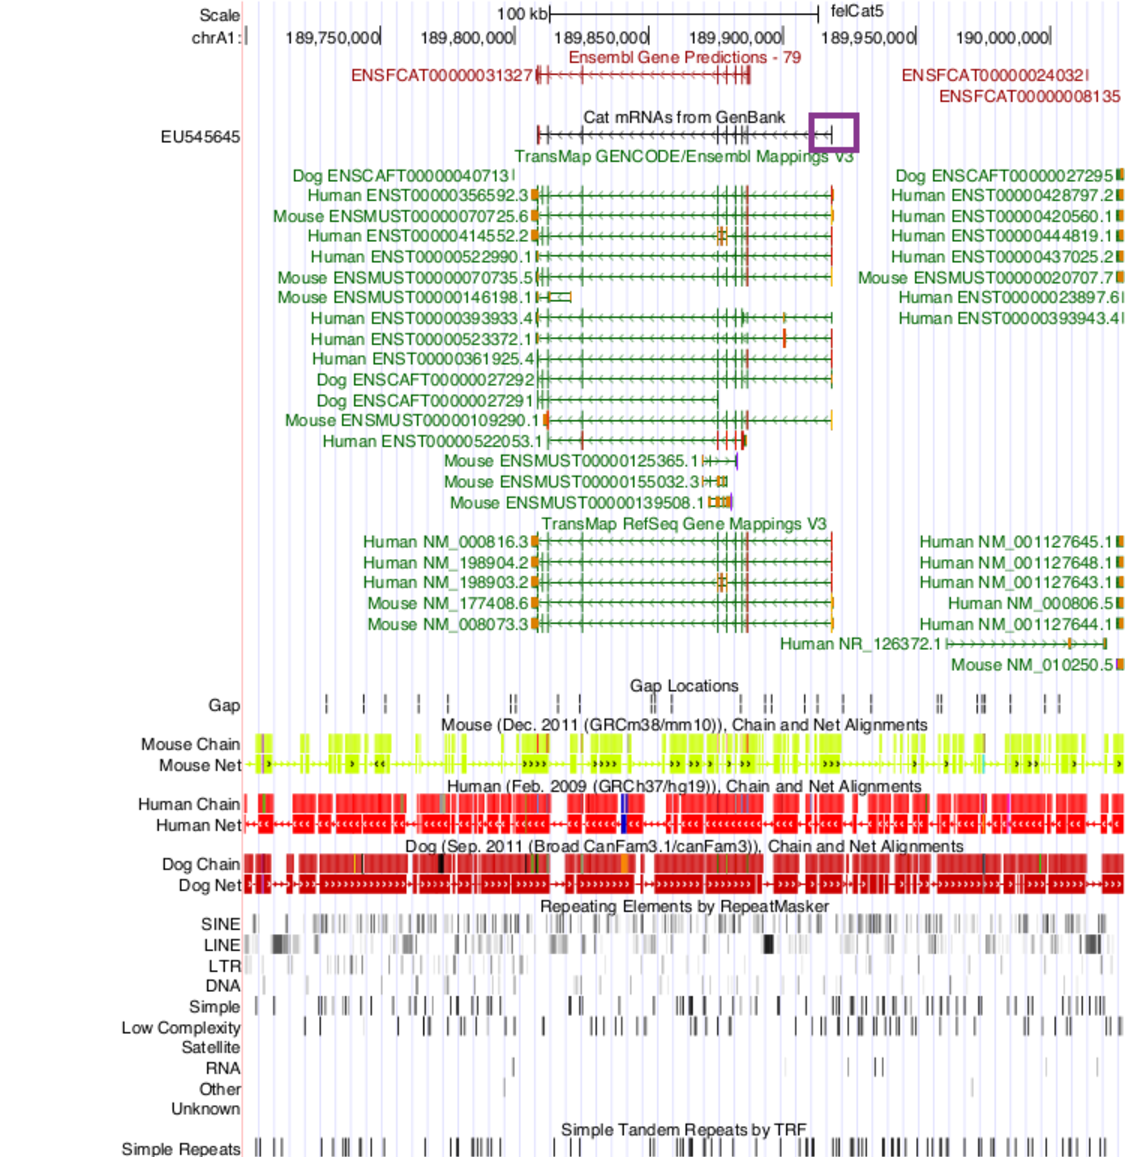
\includegraphics[width=\textwidth]{images/hgt_hgwdev_ed86_52bfa0_edit.pdf}
\caption{Another example of exon loss in gene ENSFCAT00000031327 (marked inside of the purple rectangle). Again, mRNA and TransMap are evidence of the coding region.}
\label{fig:missed_exons_mrna_2}
\end{figure}

%Figure3
\begin{figure}[h]
\centering
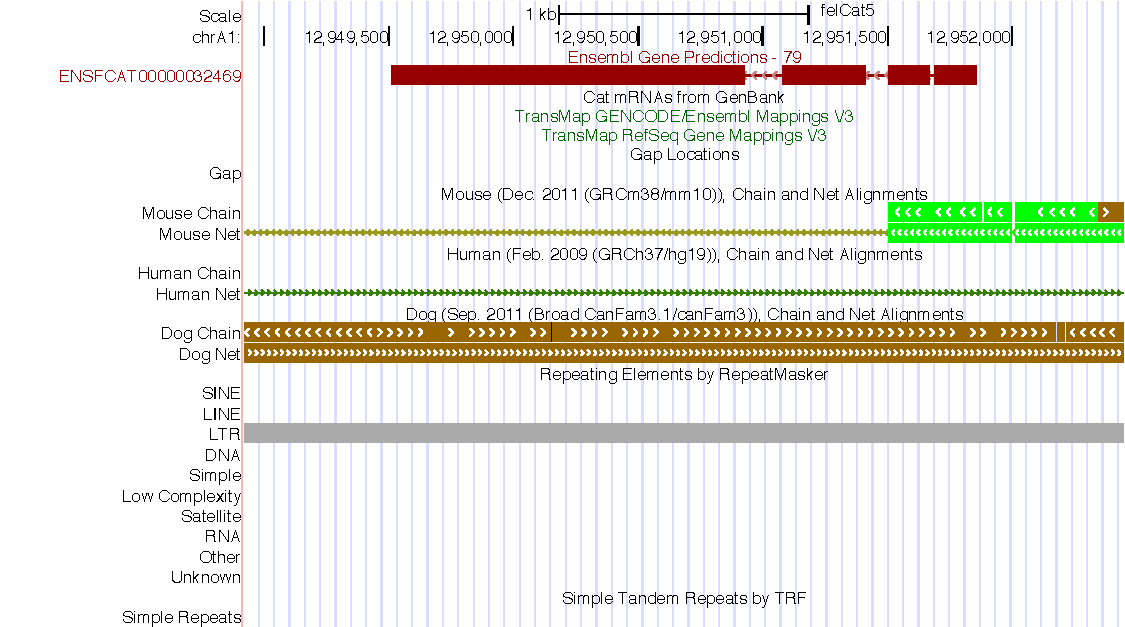
\includegraphics[width=\textwidth]{images/hgt_hgwdev_ede4_52c4e0.pdf}
\caption{Gene ENSFCAT00000032469 was predicted in the region annotated as LTR.}
\label{fig:gene_in_ltr}
\end{figure}


\subsection{RefSeq annotation}
RefSeq gene prediction is based on the alignments of the NCBI RefSeq collection of the cat RNA to the reference cat genome.

\begin{table}
\centering
\begin{tabular}{| c | c | c |}
\hline
&Ensembl&RefSeq\\

Transcripts& 22656 & 431\\

Gene clusters& 19490 & 382\\

No-error clusters & 40\% & 67.9\%\\

All-error clusters& 59\% & 30.8\%\\

Other clusters& 0.98\% & 1.0\%\\
\hline
\end{tabular}
\caption{Ensembl and RefSeq gene annotations quality.}
\label{table:ensembl_refseq_stats}
\end{table}

\section{Suggested approach}
We suggest an incorporation of Augustus guided by 
\begin{itemize}
\item Felis catus RNA-Seq data 
\item TransMap of genes predicted for human 
\end{itemize}
in order to create a newer annotation of the domestic cat genome. This approach is being used in the mouse strain project currently performed at UCSC and demonstrates the improvement of the mouse gene annotation in the different mouse strains. We are going to collaborate with Dr. Mario Stanke who developed this method and agreed to join together efforts on this work.
So we are not going to make \textit{de novo} predictions, instead the hints obtained from RNA-Seq and TransMap from human alignments will be used as the evidence for Augustus (s. Figure \ref{fig:hints_for_augustus}). 

%Figure4
\begin{figure}[h]
\centering
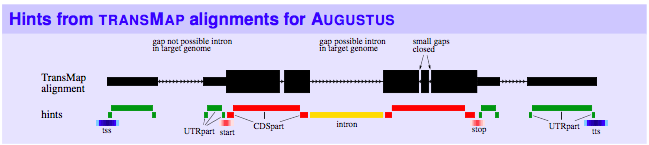
\includegraphics[width=\textwidth]{images/hints_from_transmap_to_augustus.png}
\caption{Hints from TransMap alignments for Augustus}
\label{fig:hints_for_augustus}
\end{figure}


\section{References}

\begin{enumerate}
\item Pontius, Joan U., et al. "Initial sequence and comparative analysis of the cat genome." Genome research 17.11 (2007): 1675-1689.
\item Tamazian, Gaik, et al. "Annotated features of domestic cat–Felis catus genome." GigaScience 3.1 (2014): 13.
\item Montague, Michael J., et al. "Comparative analysis of the domestic cat genome reveals genetic signatures underlying feline biology and domestication." Proceedings of the National Academy of Sciences 111.48 (2014): 17230-17235.)
\end{enumerate}


\end{document}
